\documentclass[12pt,a4paper]{article}
\usepackage[left=15mm,right=15mm,top=14mm,bottom=19mm,footskip=9mm]{geometry}
\usepackage{iftex}
\ifPDFTeX
  \usepackage[T5]{fontenc}
  \usepackage[utf8]{inputenc}
  \usepackage{mathptmx}
\else
  \usepackage{fontspec}
  \IfFontExistsTF{Times New Roman}{\setmainfont{Times New Roman}}{\setmainfont{Tinos}}
\fi
\usepackage{amsmath,amssymb}
\usepackage{tikz}
\usetikzlibrary{arrows.meta,calc}
\usepackage[most]{tcolorbox}
\usepackage{fancyhdr,lastpage}
\usepackage{tabularx,array}
\definecolor{sectionpurple}{RGB}{155,42,143}
\definecolor{notebackground}{RGB}{229,240,245}
\definecolor{noteborder}{RGB}{255,55,55}
\definecolor{graphred}{RGB}{188,55,61}
\definecolor{graphblue}{RGB}{45,95,200}
\setlength{\parindent}{0pt}
\setlength{\parskip}{2pt}
\setlength{\headheight}{15pt}
\setlength{\abovedisplayskip}{5pt}
\setlength{\belowdisplayskip}{5pt}
\setlength{\abovedisplayshortskip}{3pt}
\setlength{\belowdisplayshortskip}{3pt}
\pagestyle{fancy}
\fancyhf{}
\renewcommand{\headrulewidth}{0pt}
\renewcommand{\footrulewidth}{0.4pt}
\fancyfoot[L]{\fontsize{8.5}{10}\selectfont Tài liệu tổng hợp theo TDMXX21 (Tư Duy Mở)}
\fancyfoot[R]{\fontsize{8.5}{10}\selectfont Trang \thepage/\pageref{LastPage} -- Bài giảng 08}
\newtcolorbox{notebox}{colback=notebackground,colframe=noteborder,
  boxrule=0.8pt,arc=2pt,left=7pt,right=7pt,top=3pt,bottom=3pt,
  before skip=3pt,after skip=3pt}
\newcommand{\partheading}[1]{\par\vspace{5pt}\noindent\textbf{\textcolor{sectionpurple}{#1}}\par\vspace{1pt}}
\newcommand{\example}[2][TDM21]{\par\vspace{3pt}\noindent\textbf{\textcolor{sectionpurple}{Ví dụ #2:} \textcolor{noteborder}{[#1]}}\enspace}
\newcommand{\tightitem}{\setlength{\itemsep}{1pt}\setlength{\topsep}{1pt}\setlength{\parsep}{0pt}\setlength{\partopsep}{0pt}}
\newcommand{\veczero}{\overrightarrow{0}}
\newcommand{\cvec}[1]{\overrightarrow{#1}}
\begin{document}
\fontsize{12}{14.6}\selectfont
\begin{center}
  \textbf{BÀI GIẢNG 08}\\[-1pt]
  \textbf{CƠ BẢN VỀ KHÔNG GIAN OXYZ}\\[-2pt]
  {\fontsize{10.5}{12}\selectfont\itshape Biên soạn theo chủ đề TDMXX21 -- Tư Duy Mở}
\end{center}
\vspace{-7pt}

\partheading{PHẦN I. HỆ TỌA ĐỘ VÀ TỌA ĐỘ TRONG KHÔNG GIAN}
\textbf{1. Hệ tọa độ Oxyz}

Trong không gian cho ba trục $x'Ox$, $y'Oy$, $z'Oz$ đôi một vuông góc với nhau.
Gọi các vectơ $\vec i$, $\vec j$, $\vec k$ lần lượt là các vectơ đơn vị trên các trục $x'Ox$, $y'Oy$, $z'Oz$.
Hệ ba trục như vậy được gọi là hệ trục tọa độ Đề-các vuông góc $Oxyz$ trong không gian,
gọi đơn giản là hệ tọa độ $Oxyz$.

\begin{center}
\begin{minipage}{.47\linewidth}\centering
\begin{tikzpicture}[>=Stealth,scale=.92,line cap=round]
  \coordinate (O) at (0,0);
  \draw[->] (-2.05,-1.60)--(1.15,.90) node[above] {};
  \draw[->] (-.70,0)--(3.10,0) node[below] {$y$};
  \draw[->] (0,-1.55)--(0,2.30) node[right] {$z$};
  \node[above left] at (O) {$O$};
  \node[below] at (-2.05,-1.60) {$x$};
  \draw[->,thick] (O)--(-.79,-.62) node[below right] {$\vec i$};
  \draw[->,thick] (O)--(.91,0) node[below] {$\vec j$};
  \draw[->,thick] (O)--(0,.94) node[right] {$\vec k$};
  \draw[dashed] (-1.52,0)--(O)--(1.45,1.13);
  \fill (O) circle (1.4pt);
\end{tikzpicture}
\end{minipage}\hfill
\begin{minipage}{.47\linewidth}\centering
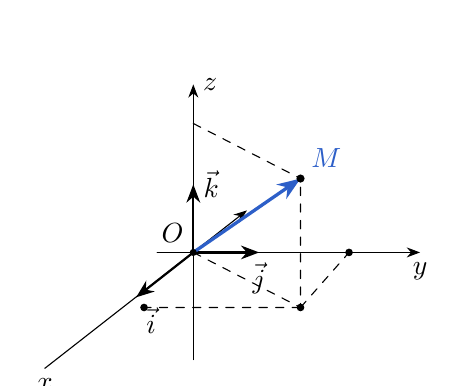
\begin{tikzpicture}[>=Stealth,scale=.92,line cap=round]
  \coordinate (O) at (0,0);
  \coordinate (P) at (1.48,-.76);
  \coordinate (M) at (1.48,1.02);
  \draw[->] (-2.05,-1.60)--(.74,.58);
  \draw[->] (-.50,0)--(3.13,0) node[below] {$y$};
  \draw[->] (0,-1.48)--(0,2.32) node[right] {$z$};
  \node[above left] at (O) {$O$};
  \node[below] at (-2.05,-1.60) {$x$};
  \draw[->,thick] (O)--(-.79,-.62) node[below right] {$\vec i$};
  \draw[->,thick] (O)--(.91,0) node[below] {$\vec j$};
  \draw[->,thick] (O)--(0,.94) node[right] {$\vec k$};
  \draw[dashed] (O)--(P)--(M);
  \draw[dashed] (P)--(-.68,-.76);
  \draw[dashed] (P)--(2.15,0);
  \draw[dashed] (0,1.78)--(M);
  \draw[->,very thick,graphblue] (O)--(M) node[above right] {$M$};
  \fill (O) circle (1.4pt);
  \fill (P) circle (1.5pt);
  \fill (M) circle (1.6pt);
  \fill (-.68,-.76) circle (1.5pt);
  \fill (2.15,0) circle (1.5pt);
\end{tikzpicture}
\end{minipage}
\end{center}
Điểm $O$ được gọi là gốc tọa độ. Các mặt phẳng $(Oxy)$, $(Oyz)$, $(Ozx)$ đôi một
vuông góc được gọi là các mặt phẳng tọa độ.
Không gian với hệ tọa độ $Oxyz$ còn được gọi đơn giản là không gian $Oxyz$.

\textbf{2. Tọa độ của điểm và tọa độ của vectơ trong không gian Oxyz}

Trong không gian $Oxyz$, cho điểm $M$ có
$\cvec{OM}=x\vec i+y\vec j+z\vec k$. Khi đó ta gọi bộ ba số $(x;y;z)$
là tọa độ của điểm $M$ và viết là $M=(x;y;z)$ hay $M(x;y;z)$.

Trong không gian $Oxyz$, cho vectơ $\vec u$ có
$\vec u=a\vec i+b\vec j+c\vec k$. Khi đó ta gọi bộ ba số $(a;b;c)$
là tọa độ của vectơ $\vec u$ và viết là $\vec u=(a;b;c)$ hay $\vec u(a;b;c)$.

Gốc tọa độ $O$ có tọa độ là $O=(0;0;0)$ vì
$\cvec{OO}=\veczero=0\vec i+0\vec j+0\vec k$.

Có $\vec i=1\vec i+0\vec j+0\vec k\Rightarrow\vec i=(1;0;0)$.
Tương tự, $\vec j=(0;1;0)$, $\vec k=(0;0;1)$.

Tọa độ các hình chiếu của điểm $M=(x;y;z)$ trên:
\begin{itemize}\tightitem
  \item Các trục tọa độ: $M_x=(x;0;0)$,\enspace $M_y=(0;y;0)$,\enspace $M_z=(0;0;z)$.
  \item Các mặt phẳng tọa độ: $M_{xy}=(x;y;0)$,\enspace
  $M_{yz}=(0;y;z)$,\enspace $M_{zx}=(x;0;z)$.
\end{itemize}

\partheading{PHẦN II. BIỂU THỨC TỌA ĐỘ CỦA CÁC PHÉP VECTƠ}
\textbf{3. Biểu thức tọa độ của các phép vectơ}

Trong không gian $Oxyz$, cho hai vectơ $\vec u=(a;b;c)$,
$\vec v=(a';b';c')$ và số thực $k$. Ta có:
\[
 \vec u\pm\vec v=(a\pm a';\,b\pm b';\,c\pm c'),\qquad
 k\vec u=k(a;b;c)=(ka;kb;kc).
\]
\textbf{Hệ quả:}
\[
 \vec u=\vec v\iff
 \begin{cases}a=a'\\ b=b'\\c=c'\end{cases};
 \qquad \veczero=(0;0;0).
\]
Cho $\vec v\ne\veczero$, hai vectơ $\vec u,\vec v$ cùng phương khi và chỉ khi
có số thực $k$ sao cho
\[
 \vec u=k\vec v\iff
 \begin{cases}a=ka'\\b=kb'\\c=kc'\end{cases}.
\]
Ba điểm phân biệt $A,B,C$ thẳng hàng khi và chỉ khi có số thực $k$
sao cho $\cvec{AB}=k\cvec{AC}$.

Tọa độ của điểm $M$ cũng chính là tọa độ của vectơ $\cvec{OM}$:
$M=(x;y;z)\iff\cvec{OM}=(x;y;z)$.

Cho $A=(x_A;y_A;z_A)$, $B=(x_B;y_B;z_B)$, $C=(x_C;y_C;z_C)$. Ta có:
\[
 \cvec{AB}=\cvec{OB}-\cvec{OA}
 =(x_B-x_A;\,y_B-y_A;\,z_B-z_A).
\]
Tọa độ trung điểm $I$ của đoạn $AB$:
\[
 I=\left(\frac{x_A+x_B}{2};\frac{y_A+y_B}{2};\frac{z_A+z_B}{2}\right).
\]
Tọa độ trọng tâm $G$ của tam giác $ABC$:
\[
 G=\left(\frac{x_A+x_B+x_C}{3};
          \frac{y_A+y_B+y_C}{3};
          \frac{z_A+z_B+z_C}{3}\right).
\]
Điểm $N$ (gọi là tâm tỉ cự) thỏa mãn
$\alpha\cvec{NA}+\beta\cvec{NB}+\gamma\cvec{NC}=\veczero$
(với $\alpha+\beta+\gamma\ne0$) có tọa độ:
\[
 N=\frac{\alpha A+\beta B+\gamma C}{\alpha+\beta+\gamma}
 \quad\text{(hiểu theo từng tọa độ).}
\]

\begin{notebox}
\example[TDM31]{01} Trong không gian $Oxyz$, cho các điểm
$A=(1;2;3)$, $B=(3;0;-1)$, $C=(-1;4;-2)$. Hãy xác định:
\begin{enumerate}\tightitem
 \item Tọa độ các điểm là hình chiếu của $A$ trên các trục và các mặt phẳng tọa độ.
 \item Tọa độ trung điểm $I$ của đoạn $AB$.
 \item Tọa độ trọng tâm $G$ của tam giác $ABC$.
 \item Tọa độ điểm $D$ sao cho tứ giác $ABCD$ là hình bình hành.
 \item Tọa độ điểm $M=AB\cap(Oxy)$.
 \item Tọa độ điểm $N$ thỏa mãn $\cvec{NA}+2\cvec{NB}=\veczero$.
\end{enumerate}
\end{notebox}

\partheading{PHẦN III. TÍCH VÔ HƯỚNG VÀ ỨNG DỤNG}
\textbf{4. Tích vô hướng và ứng dụng}

\textbf{Biểu thức tọa độ của tích vô hướng:}
Trong không gian $Oxyz$, tích vô hướng của hai vectơ
$\vec u=(a;b;c)$ và $\vec v=(a';b';c')$ được xác định bởi công thức:
\[
 \vec u\cdot\vec v=aa'+bb'+cc'.
\]
\textbf{Hệ quả:} Độ dài vectơ $\vec u=(a;b;c)$:
\[
 |\vec u|=\sqrt{a^2+b^2+c^2}.
\]
Độ dài đoạn thẳng $AB$:
\[
 AB=|\cvec{AB}|=
 \sqrt{(x_B-x_A)^2+(y_B-y_A)^2+(z_B-z_A)^2}.
\]
Cho hai vectơ $\vec u=(a;b;c)$, $\vec v=(a';b';c')$ khác $\veczero$.
Khi đó góc giữa hai vectơ thỏa mãn:
\[
 \vec u\cdot\vec v=|\vec u|\,|\vec v|\,\cos(\vec u,\vec v)
 \quad\Rightarrow\quad
 \cos(\vec u,\vec v)=
 \frac{\vec u\cdot\vec v}{|\vec u|\,|\vec v|}
 =\frac{aa'+bb'+cc'}
 {\sqrt{a^2+b^2+c^2}\sqrt{a'^2+b'^2+c'^2}}.
\]
Và:
\[
 \vec u\perp\vec v
 \iff\vec u\cdot\vec v=0
 \iff aa'+bb'+cc'=0.
\]

\begin{notebox}
\example[TDM21]{01} Trong không gian $Oxyz$, cho
$\vec u=2\vec i+3\vec j-4\vec k$, $\vec v=(2;2;1)$, $\vec w=(m;1;2)$.
Hãy tính $\vec u\cdot\vec v$, $\cos(\vec u,\vec v)$.
Hãy tìm $m$ để $\vec u\perp\vec w$.
\end{notebox}

\begin{notebox}
\example[TDM32]{02} Trong không gian $Oxyz$, cho các điểm
$A=(0;1;2)$, $B=(2;2;4)$, $C=(0;-2;-2)$.
Hãy xác định diện tích, bán kính đường tròn ngoại tiếp và bán kính
đường tròn nội tiếp của tam giác $ABC$.
\end{notebox}

\begin{center}
\textbf{\textcolor{sectionpurple}{--- Hết ---}}
\end{center}
\end{document}
